\documentclass[twoside]{article}
\usepackage[accepted]{aistats2017}
\usepackage{amsmath,amsthm,amssymb,amsfonts}
\usepackage{graphicx}

 % If your paper is accepted, change the options for the package
% aistats2017 as follows:
%
%\usepackage[accepted]{aistats2017}
%
% This option will print headings for the title of your paper and
% headings for the authors names, plus a copyright note at the end of
% the first column of the first page.


\begin{document}

% If your paper is accepted and the title of your paper is very long,
% the style will print as headings an error message. Use the following
% command to supply a shorter title of your paper so that it can be
% used as headings.
%
%\runningtitle{I use this title instead because the last one was very long}

% If your paper is accepted and the number of authors is large, the
% style will print as headings an error message. Use the following
% command to supply a shorter version of the authors names so that
% they can be used as headings (for example, use only the surnames)
%
%\runningauthor{Surname 1, Surname 2, Surname 3, ...., Surname n}

\twocolumn[

\aistatstitle{The Evaluation of Parameter Estimator for Simple Linear Model}

\aistatsauthor{ Yihong Gu }

\aistatsaddress{ Department of Computer Science \\ Tsinghua University \\ gyh15@mails.tsinghua.edu.cn} ]

\begin{abstract}

In this paper, we get in the model of simple linear regression and proposed five main estimators of it. Then we carefully analyse the estimators' intuitive behaviour and calcuate their analytical or numerical solution. We then design the experiments, especially in data generation. We expose the estimator to different kind of pseudo-data designed above and generated by R and anaylse its performance in four main perspectives: minumum variance, bias, consistence and large sample property. Finally we visualize the fitted line of these estimators and demonstrate the intuitive understanding of the five estimators.

\end{abstract}

\section{Model}

We evaluate the performance of some parameter estimators for Simple Linear Model. We consider the simplest case, in which we are given the data set $\{(x_i,y_i)\}_{i=1}^n$, where the $x_i$'s and $y_i$'s are all real number in $\mathbb{R}^1$, the probabilistic model is

\begin{eqnarray}
  Y_i = a X_i + b + \epsilon_i
\end{eqnarray}

where $i \in \{1, 2,\cdots, n\}$, $Y_i, \epsilon_i$ are all random variables, and $X_i$ is a constant when $i$ is fixed. At the same time, $a$ and $b$ are the parameter we want to estimate. We call $X_i$ \textbf{explanatory variable} and call $Y_i$ \textbf{response variable}, while $\epsilon_i$ is a random error that can't be measured exactly.
We regard this model as a discriminant model instead of a generative one (although in reality the explanatory variable $X$ might has distribution itself but for simplicity we ignore it).

In the perspective of expectation, we add more constraints on the model

\begin{eqnarray}
  \mathbb{E}[Y_i\lvert X=X_i] &=& a X_i + b + \mathbb{E}[\epsilon_i\lvert X=X_i] \\
  &=& a X_i + b
\end{eqnarray}

Here, we assume $\mathbb{E}[\epsilon_i\lvert X=X_i]=0$ for any $X_i$ and $\epsilon_i$ are i.i.d.

For summary, we define our model through 4 steps:

\begin{itemize}
  \item (constant) explanatory variable: $X_i$
  \item parameters: $a$(slope) and $b$(intercept)
  \item i.i.d. noise random variable: $\epsilon_1, \cdots, \epsilon_n$
  \item response variable: $Y_i = a X_i + b + \epsilon_i$
\end{itemize}

When the model is clearly defined, we are given the data set $\mathcal{D}=\{(x_i,y_i)\}_{i=1}^n$, and use $\mathcal{D}$ to estimate the parameters $a$ and $b$.

\section{Method}

We suppose there exsits the true parameter $a^*$ as well as $b^*$ and the data are sampled according the model. In order to estimate the true parameter through data set $\mathcal{D}$, intuitively we want to use a straight line to fit the points $(x_i, y_i)$ and let the total distance from the points to the line be as small as possible. The central question here is that how can we define the 'distance', we consider the following 5 total distances

\begin{itemize}
  \item $G_1(a,b)=\frac{1}{n}\sum_{i=1}^n{\lvert y_i - a x_i - b\rvert}$
  \item $G_2(a,b)=\frac{1}{n}\sum_{i=1}^n{(y_i- a x_i - b)^2}$
  \item $G_3(a,b)=\max_{1 \le i\le n}{\lvert y_i - a x_i - b\rvert}$
  \item $G_4(a,b)=\frac{1}{n}\sum_{i=1}^n{(x_i-\frac{y_i-b}{a})^2}$
  \item $G_5(a,b)=\frac{1}{n}\sum_{i=1}^n{\frac{(y_i-a x_i - b)^2}{1+a^2}}$
\end{itemize}

So we then covert the origin estimate problem to a optimization problem: for a particular distance measurement $G_i(a,b)$, we find the parameter $\hat{a}, \hat{b}$ that minimize the total distance $G_i(a,b)$ and let it to estimate the parameter. In the following sections we call $G_i(a,b)$ \textbf{object function}.

In the following subsections we discuss the intuition behind each object function and optimize them via analytical or numerical methods

\subsection{Least Square Estimator}

Firstly we jointly discuss the behaviour and optimization of $G_2(a,b)$, $G_4(a,b)$ and $G_5(a,b)$. In order to get a intuitive understanding of these 'Least Square' object function, we suppose we fix the variable $a$ and want to find the optimal $b$ according to $a$, it might be clear that our object function can be written as the following form (\ref{lsef2})(\ref{lsef4})(\ref{lsef5})

\begin{eqnarray}
\label{lsef2}
G_2(a,b) &=& \frac{1}{n} \sum_{i=1}^n{(u_i - b)^2} \\
\label{lsef4}
G_4(a,b) &=& \frac{1}{n} \sum_{i=1}^n{\big(\frac{u_i - b}{a}\big)^2} \\
\label{lsef5}
G_5(a,b) &=& \frac{1}{n} \sum_{i=1}^n{\frac{1}{a^2+1}(u_i-b)^2}
\end{eqnarray}

where 

\begin{eqnarray}
u_i = y_i - a x_i
\end{eqnarray}

these re-form mainly make two main contributions to our work. Firstly, we can see that, the least square object function might optimize the mean square error of the distance, here it should be emphasized that the distance vary in different forms: vertical distance ($G_2$), horizontal distance ($G_4$), perpendicular distance ($G_5$). Moreover we can get the optimal $b$ when $a$ is fixed:

\begin{eqnarray}
\label{optb}
\hat{b} = \bar{y} - a \bar{x}
\end{eqnarray}

where $\bar{y}$, $\bar{x}$ are the sample mean of $\{x_i\}_{i=1}^n$ and $\{y_i\}_{i=1}^n$, so using simple calculus, we can derived the optimal $a, b$.

The optimal $a, b$ for vertical least square object function (VLSE) is

\begin{eqnarray}
  \hat{a}^{VLSE} &=& \frac{\sum_{i=1}^n{(y_i-\bar{y})(x_i-\bar{x})}}{\sum_{i=1}^n{(x_i-\bar{x})^2}} \\
  \hat{b}^{VLSE} &=& \bar{y} - \hat{a}^{VLSE} \bar{x}
\end{eqnarray}

The optimal $a, b$ for horizontal least square object function (HLSE) is

\begin{eqnarray}
  \hat{a}^{HLSE} &=& \frac{\sum_{i=1}^n{(y_i-\bar{y})^2}}{\sum_{i=1}^n{(y_i-\bar{y})(x_i-\bar{x})}} \\
  \hat{b}^{HLSE} &=& \bar{y} - \hat{a}^{HLSE} \bar{x}
\end{eqnarray}

The optimal $a, b$ for perpendicular least square object function (PLSE) is 

\begin{eqnarray}
  \hat{a}^{PLSE} &=& \frac{\sum_{i=1}^n{(y_i-\bar{y})^2}-(x_i-\bar{x})^2}{2\sum_{i=1}^n{(y_i-\bar{y})(x_i-\bar{x})}} \nonumber \\ &+& \sqrt{1+\big[\frac{\sum_{i=1}^n{(y_i-\bar{y})^2}-(x_i-\bar{x})^2}{2\sum_{i=1}^n{(y_i-\bar{y})(x_i-\bar{x})}}\big]^2} \label{bb} \\
  \hat{b}^{PLSE} &=& \bar{y} - \hat{a}^{PLSE} \bar{x}
\end{eqnarray}

We want to emphasize that this equation (\ref{bb}) holds when the sample correlation of $X$ and $Y$ is greater than 0.

We also use the numerical method to check whether our derivation of the closed forms of VLSE and PLSE are right, so we calculate the partial gradients, which are as followings:

\begin{eqnarray}
  \frac{\partial G_4}{\partial a}&=&\frac{2}{n}\sum_{i=1}^n{(x_i-\frac{y_i-b}{a})\frac{y_i-b}{a^2}} \\
  \frac{\partial G_4}{\partial b}&=&\frac{2}{n}\sum_{i=1}^n{(x_i-\frac{y_i-b}{a})\frac{1}{a}} \\
  \frac{\partial G_5}{\partial a}&=&\frac{2\sum_{i=1}^n{(y_i-a x_i-b)(-x_i-a y_i-b)}}{n(a^2+1)^2} \\
  \frac{\partial G_5}{\partial b}&=&\frac{-2\sum_{i=1}^n{(y_i-a x_i-b)}}{n(a^2+1)^2}
\end{eqnarray}

\subsection{Least Absolute Deviation}
\label{lad}

We understand the object function (\ref{ladof}) intuitively through a very simple reduction vision, in which we assume $a=0$, so the optimal $b$ is the median of all the $y_i$'s, so the optimal solution for the object function (\ref{ladof}) might somewhat be a 'median optimization', which might perfer to estimate close to the 'median'

\begin{eqnarray}
\label{ladof}
  G_1(a,b)=\frac{1}{n}\sum_{i=1}^n{\lvert y_i - a x_i - b\rvert}
\end{eqnarray}

The optimal solution don't have closed form, so we use numerical method to get the optimal solution and the gradient is

\begin{eqnarray}
  \frac{\partial G_1}{\partial a}&=&\frac{1}{n}\sum_{i=1}^n{\mathrm{sign}(y_i-a x_i - b)(-x_i)} \\
  \frac{\partial G_1}{\partial b}&=&\frac{1}{n}\sum_{i=1}^n{\mathrm{sign}(y_i-a x_i - b)(-1)} 
\end{eqnarray}

where we define

\begin{eqnarray}
\mathrm{sign}(x) = 1_{x>0} - 1_{x<0}
\end{eqnarray}

\subsection{Least Maximum Estimate}

We understand the object function (\ref{lmeof}) using the similiar method describe in (\ref{lad}), we suppose $a=0$, and find that the optimal $b$ will strike a balance between the maximum and the minimum value of $y$, so we found that the least maximum estimate might find a solution that in the 'middle' of the minimum and the maximum 'situation'.

\begin{eqnarray}
\label{lmeof}
G_3(a,b)=\max_{1 \le i\le n}{\lvert y_i - a x_i - b\rvert}
\end{eqnarray}

The optimal solution also don't have closed form, so we compute the gradients:

\begin{eqnarray}
  \frac{\partial G_3}{\partial a}&=&(y_k-a x_k - b)(-x_k) \\
  \frac{\partial G_3}{\partial b}&=&(y_k-a x_k - b)(-1) 
\end{eqnarray}

where $k = \mathrm{argmax}_i \lvert y_i - a x_i - b\rvert$

\section{Evaluation}

\subsection{Data Generation}

\label{process}

Following the setting of our model, we perform our experiment in the following steps:

\begin{itemize}
  \item[1.] We set the true value of the parameter to be $a=1, b=2$ and use the true value to generate pseudo data, and then use the pseudo data and different estimators to estimate the parameters.
  \item[2.] We set the data size $n=30, 100, 1000$, and see how the estimators performed under diffenent scales of data.
  \item[3.] We design $\{x_i\}_{i=1}^n$. We can generate $x$ randomly or fixedly, here we consider two classic methods:
        \item Let $x_i \sim\text{ }\mathrm{i.i.d}\textbf{ }\mathcal{U}[0, 1]$
        \item Make $x_i$ have same distance, i.e. let $x_i = \frac{i}{n}$.
  \item[4.] Set the noise, we also consider 2 major settings:
        \item $\epsilon_1, \cdots, \epsilon_n \sim\text{ }\mathrm{i.i.d.} \text{ }\mathcal{N}(0,\sigma^2)$, where $\sigma=0.1,1,2$
        \item $\epsilon_1, \cdots, \epsilon_n \sim\text{ }\mathrm{i.i.d.} \text{ }\mathrm{Cauchy}(0,\xi)$, where $\xi=0.1$
        \item $\epsilon_1, \cdots, \epsilon_n \sim\text{ }\mathrm{i.i.d.} \text{ }\mathcal{U}(-\sigma,\sigma)$, where $\sigma=0.2$
  \item[5.] We use the model $Y_i=a X_i + b + \epsilon_i$ and the generated value $\{x_i\}_{i=1}^n$ and $\{\epsilon_i\}_{i=1}^n$ to calculate $\{y_i\}_{i=1}^n$, so here now we have the data $\{(x_i,y_i)\}_{i=1}^n$.
  \item[6.] We use the data and different estimators ($G_1,\cdots,G_5$) to estimate $(\hat{a}_1,\hat{b}_1),\cdots,(\hat{a}_5,\hat{b}_5)$ and see how they vary from the true value ($a$,$b$)
\end{itemize}

We repeat [2]$\sim$[6] $T$ times and generate $\{(\hat{a}_1^{(t)},\hat{b}_1^{(t)})\}_{t=1}^T$, $\{(\hat{a}_2^{(t)},\hat{b}_2^{(t)})\}_{t=1}^T$, $\{(\hat{a}_3^{(t)},\hat{b}_3^{(t)})\}_{t=1}^T$, $\{(\hat{a}_4^{(t)},\hat{b}_4^{(t)})\}_{t=1}^T$, $\{(\hat{a}_5^{(t)},\hat{b}_5^{(t)})\}_{t=1}^T$ and see how they separately distributed. Evaluate whether it is unbiased and see their variance and MSE. 

\subsection{Implemention Details}

We used 'optim' function to get a numerical solution 

We used both numerical and analytical method for horizontal least square estimator (HLSE) and perpendicular least square estimator (PLSE) and check whether the estimate they given are different, we found that their relative error is under 0.05 when we use noise $\mathcal{N}(0,0.1)$ and $\mathcal{U}(-0.2,0.2)$ and might be larger than it when use other noise options, however, we found analytical method always provide a better soluton (provided a lower loss), so we always uses analytical method for HLSE and PLSE.

Moreover, we fixed the random seed to be 123469 and use R-package 'ggplot2' to generate plots and 'xtable' to directly convert data.frame in R to table format in Latex.

\section{Experiments and Results}

We execute experiments through the process describe in Subsection \ref{process}, and the full results of estimate bias and standard deviation in Appendix \ref{append}, here we discuss our results of expriements and analyse it in two major perspectives. Firstly, we discuss the summary performance of different estimators in difference noise/explanatory variable distribution options and see which estimator outperform others in different situations. Moreover, we provided some visualization about samples of fitted line of different estimators and see their characteristics.

\subsection{Overall Analysis}

\subsubsection*{Normal distributed noise}

We found that the distribution of the estimator don't have significant difference whether $X$ is distrbuted fixedly or unifomly when the noise is normal distributed, so we only uses uniformly distributed $X$ to give the following analysis.

We quickly overview the following properties:

\begin{itemize}
  \item [1.] \textbf{MVUE}: VLSE outperform all other estimators, which has the lowest variance.
  \item [2.] \textbf{Bias}: VLSE, VLAD and VLME are both unbiased estimators, and HLSE and PLSE will over-estimate slope $a$ and under-estimate $b$.
\end{itemize}

When the variance of noise is low ($\sigma=0.1$), we can see how their perform in the boxplot Figure \ref{30-normal-0.1}

\begin{center}
\makeatletter
\def\@captype{figure}
\makeatother
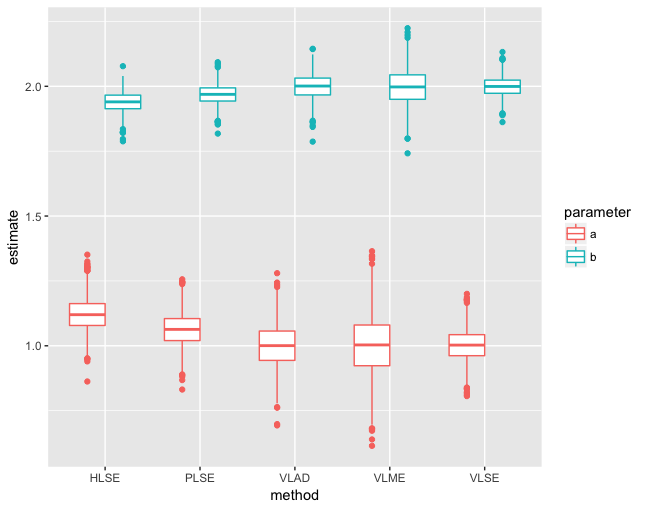
\includegraphics [height=7cm]{code/n=30,uniform,normal_0.1.png}
\caption{Boxplot of estimators, $\epsilon \sim \mathcal{N}(0,0.1)$, $n=30$}
\label{30-normal-0.1}
\end{center}

When the variance is quite high ($\sigma=2$), we can see the performance of HSLE and PSLE will be quite poor (for example, even $n=1000$, large sample), the boxplot show in Figure \ref{1000-normal-2}

\begin{center}
\makeatletter
\def\@captype{figure}
\makeatother
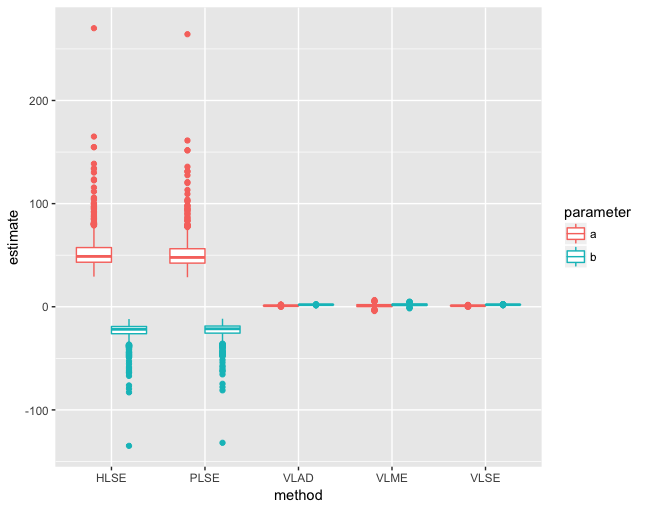
\includegraphics [height=7cm]{code/n=1000,uniform,normal_2.png}
\caption{Boxplot of estimators, $\epsilon \sim \mathcal{N}(0,2)$, $n=1000$}
\label{1000-normal-2}
\end{center}

When we focus only on the three unbiased estimaor, we can see how they perform in boxplot Figure \ref{1000-normal-2-3}, in which VLSE perform slightly better than VLAD, and both of them outperform VLME largely

\begin{center}
\makeatletter
\def\@captype{figure}
\makeatother
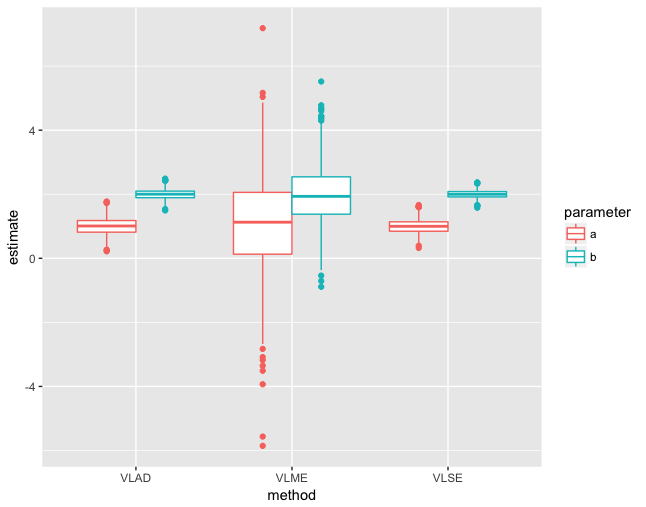
\includegraphics [height=7cm]{code/special/n=1000,uniformed,normal_2,3.png}
\caption{Boxplot of unbiased estimators, $\epsilon \sim \mathcal{N}(0,2)$, $n=1000$}
\label{1000-normal-2-3}
\end{center}

We found the consistency and large sample property of these estimators are similar no matter how $\sigma$ vary, and give the conclusion as followings:

\begin{itemize}
  \item [3.] \textbf{Consistency}: Regardless of how $\sigma$ changes, we found VLAD, VLSE both has consistency property, and the variance of VLME don't vary when sample size increases. Moreover HLSE, PLSE are still biased then sample size is very large.
  \item [4.] \textbf{Large Sample Property}: Regardless of how $\sigma$ changes, we found VLAD, VLSE, HLSE, PLSE's variance decreases when sample size increases, while the variance of VLME don't vary very much.
\end{itemize}

\subsubsection*{Cauchy distributed noise}

Two major statistics of cauchy distributed noises are as followings in Table \ref{cu} and \ref{cf}

\begin{table}[ht]
\centering
\caption{fixed $X$, $\epsilon \sim \mathrm{Cauchy}(0,0.1)$}
\begin{tabular}{rlrrrr}
  \hline
 & method & a.bias & a.sd & b.bias & b.sd \\ 
  \hline
  30 & VLAD & \textbf{0.002} & \textbf{0.108} & \textbf{-0.004} & \textbf{0.062} \\ 
  30 & VLSE & 0.139 & 9.132 & -0.096 & 6.586 \\ 
  30 & VLME & -0.063 & 7.436 & -0.185 & 34.296 \\ 
  30 & HLSE & -45.118 & 2467.1 & 22.533 & 1233.7 \\ 
  30 & PLSE & -44.808 & 2443.8 & 22.378 & 1222.0 \\ 
  \hline
  100 & VLAD & \textbf{-0.001} & \textbf{0.054} & \textbf{-0.001} & \textbf{0.031} \\ 
  100 & VLSE & 0.580 & 26.369 & -0.604 & 19.531 \\ 
  100 & VLME & 0.268 & 13.460 & -15.605 & 351.753 \\ 
  100 & HLSE & -22.683 & 2885.6 & 11.028 & 1447.11 \\ 
  100 & PLSE & -23.212 & 2884.3 & 11.292 & 1446.43 \\ 
  \hline
  1000 & VLAD & \textbf{-0.001} & \textbf{0.017} & \textbf{0.001} & \textbf{0.010} \\ 
  1000 & VLSE & -1.667 & 26.787 & 0.423 & 11.228 \\ 
  1000 & VLME & 15.23 & 781.16 & -207.35 & 5981.57 \\ 
  1000 & HLSE & -4363.2 & 70387 & 2181.2 & 35184 \\ 
  1000 & PLSE & -4363.6 & 70384 & 2181.4 & 35182 \\ 
  \hline
\end{tabular}
\label{cu}
\end{table}

We found that the distribution and especially summary statistics of the estimator don't have significant difference whether $X$ is distrbuted fixedly or unifomly when the noise is normal distributed, so we only uses uniformly distributed $X$ to give the following analysis.

\begin{itemize}
  \item [1.] \textbf{MVUE}: VLAD outperform all other estimators, which has the lowest variance.
  \item [2.] \textbf{Bias}: We think only VLAD is the only unbiased estimator, the other four estimates even don't have expectations due to that Cauchy distribution don't have expectations itself.
\end{itemize}

Due to Cauchy distribution don't have expectation, so the sample standard deviation and mean statistics don't offer information (Because they don't exsits, so the Weak Large Number Law don't holds). But we can see that the estimates VLSE and VLME offered might be close to the true value while HLSE and PLSE don't have such properties.

\begin{table}[ht]
\centering
\caption{uniform $X$, $\epsilon \sim \mathrm{Cauchy}(0,0.1)$}
\begin{tabular}{rlrrrr}
  \hline
 & method & a.bias & a.sd & b.bias & b.sd \\ 
  \hline
  30 & VLAD & -0.004 & \textbf{0.117} & \textbf{0.001} & \textbf{0.067 }\\ 
  30 & VLSE & \textbf{0.003} & 6.052 & -0.126 & 4.318 \\ 
  30 & VLME & -0.007 & 8.944 & -1.968 & 33.145 \\ 
  30 & HLSE & 32.848 & 768.75 & -17.232 & 422.26 \\ 
  30 & PLSE & 31.735 & 759.24 & -16.654 & 417.09 \\ 
  \hline
  100 & VLAD & \textbf{-0.000} & \textbf{0.057} & \textbf{-0.001} & \textbf{0.033} \\ 
  100 & VLSE & 0.72 & 20.48 & -0.52 & 13.63 \\ 
  100 & VLME & -1.43 & 46.81 & -8.07 & 215.15 \\ 
  100 & HLSE & -73.27 & 6359.5 & 29.28 & 3140.5 \\ 
  100 & PLSE & -72.63 & 6320.1 & 28.98 & 3121.9 \\ 
  \hline
  1000 & VLAD & \textbf{0.00} & \textbf{0.02} & \textbf{-0.00} & \textbf{0.01} \\ 
  1000 & VLSE & -0.86 & 17.71 & 0.09 & 5.16 \\ 
  1000 & VLME & 9.84 & 127.85 & -167.75 & 2875.86 \\ 
  1000 & HLSE & -945.37 & 35303. & 467.74 & 17710. \\ 
  1000 & PLSE & -946.17 & 35303. & 468.15 & 17710. \\ 
  \hline
\end{tabular}
\label{cf}
\end{table}

\subsubsection*{Uniform distributed noise}

Two major statistics of cauchy distributed noises are as followings in Table \ref{uf} and \ref{uu}

\begin{table}[ht]
\centering
\caption{fixed $X$, $\epsilon \sim \mathcal{U}(-0.2,0.2)$}
\begin{tabular}{rlrrrr}
  \hline
 & method & a.bias & a.sd & b.bias & b.sd \\ 
  \hline
  30 & VLAD & -0.008 & 0.113 & 0.006 & 0.066 \\ 
  30 & VLSE & -0.003 & 0.070 & 0.003 & 0.040 \\ 
  30 & VLME & \textbf{0.000} & \textbf{0.046} & \textbf{-0.000} & \textbf{0.026} \\ 
  30 & HLSE & 0.138 & 0.066 & -0.068 & 0.038 \\ 
  30 & PLSE & 0.069 & 0.071 & -0.033 & 0.041 \\ 
  \hline
  100 & VLAD & 0.002 & 0.069 & 0.001 & 0.039 \\ 
  100 & VLSE & 0.001 & 0.041 & 0.000 & 0.023 \\ 
  100 & VLME & \textbf{0.000} & \textbf{0.016} & \textbf{-0.000} & \textbf{0.009} \\ 
  100 & HLSE & 0.156 & 0.038 & -0.077 & 0.022 \\ 
  100 & PLSE & 0.081 & 0.042 & -0.040 & 0.024 \\ 
  \hline
  1000 & VLAD & 0.001 & 0.022 & -0.001 & 0.012 \\ 
  1000 & VLSE & 0.001 & 0.012 & -0.000 & 0.007 \\ 
  1000 & VLME & \textbf{-0.000} & \textbf{0.002} & \textbf{0.000} & \textbf{0.001} \\ 
  1000 & HLSE & 0.160 & 0.012 & -0.080 & 0.007 \\ 
  1000 & PLSE & 0.084 & 0.013 & -0.042 & 0.007 \\ 
   \hline
\end{tabular}
\label{uf}
\end{table}

\begin{table}[ht]
\centering
\caption{uniform $X$, $\epsilon \sim \mathcal{U}(-0.2,0.2)$}
\begin{tabular}{rlrrrr}
  \hline
 & method & a.bias & a.sd & b.bias & b.sd \\ 
  \hline
  30 & VLAD & \textbf{0.000} & 0.123 & \textbf{0.000} & 0.071 \\ 
  30 & VLSE & 0.001 & 0.077 & -0.001 & 0.045 \\ 
  30 & VLME & \textbf{-0.000} & \textbf{0.052} & \textbf{-0.000} & \textbf{0.030} \\ 
  30 & HLSE & 0.160 & 0.076 & -0.081 & 0.045 \\ 
  30 & PLSE & 0.083 & 0.079 & -0.042 & 0.046 \\
  \hline
  100 & VLAD & \textbf{0.001} & 0.070 & \textbf{0.000} & 0.040 \\ 
  100 & VLSE & \textbf{0.001} & 0.042 & \textbf{0.000} & 0.024 \\ 
  100 & VLME & \textbf{-0.001} & \textbf{0.017} & 0.001 & \textbf{0.010} \\ 
  100 & HLSE & 0.162 & 0.041 & -0.080 & 0.024 \\ 
  100 & PLSE & 0.085 & 0.043 & -0.041 & 0.024 \\  
  \hline
  1000 & VLAD & -0.001 & 0.022 & \textbf{0.000} & 0.013 \\ 
  1000 & VLSE & -0.001 & 0.013 & \textbf{0.000} & 0.007 \\ 
  1000 & VLME & \textbf{-0.000} & \textbf{0.002} & \textbf{0.000} & \textbf{0.001} \\ 
  1000 & HLSE & 0.159 & 0.013 & -0.080 & 0.008 \\ 
  1000 & PLSE & 0.083 & 0.013 & -0.041 & 0.008 \\ 
   \hline
\end{tabular}
\label{uu}
\end{table}

We found that the distribution of the estimator might have slightly difference whether $X$ is distrbuted fixedly or unifomly when the noise is uniformed distributed:

\begin{itemize}
  \item [0.] The variance might be lower when $X$ is distributed fixedly than is distributed uniformly
\end{itemize}

Also overviewing the following properties:

\begin{itemize}
  \item [1.] \textbf{MVUE}: VLME outperform all other estimators, which has the lowest variance.
  \item [2.] \textbf{Bias}: VLSE, VLAD and VLME are both unbiased estimators, and HLSE and PLSE will over-estimate slope $a$ and under-estimate $b$.
\end{itemize}

Take the boxplot of $n=100$ as a example, we can see VLME has a sailent advanage over other estimates.

\begin{center}
\makeatletter
\def\@captype{figure}
\makeatother
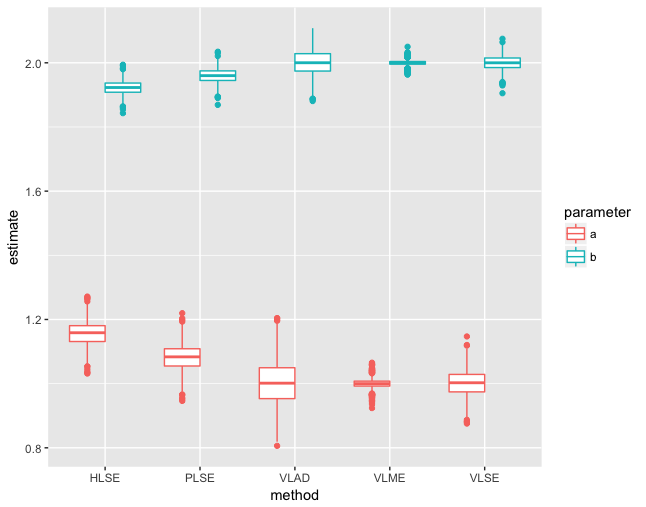
\includegraphics [height=7cm]{code/n=100,fixed,uniform.png}
\caption{Boxplot of estimators, $\epsilon \sim \mathcal{U}(-0.2,0.2)$, $n=100$}
\label{100-fixed-uniform}
\end{center}

\begin{itemize}
  \item [3.] \textbf{Consistency}: We found VLAD, VLSE, VLME both has consistency property. Moreover HLSE, PLSE are still biased then sample size is very large.
  \item [4.] \textbf{Large Sample Property}: We found all the estimators' variances decrease when sample size increases.
\end{itemize}

\subsection{Fitted Line Visualization}

Here we visualize the fitted line of the five estimators. For unity, we use uniformly distributed $X$ and $n=100$.

We uses black line to represent the true value, red for VLSE, orange for VLAD, green for VLME, blue for HLSE and purple for PLSE.

The first plot  Figure \ref{normal_0.1} uses noise $\sim \mathcal{N}(0,0.1)$. We can see all the estimators give similiar and good estimate due to the low noise.

\begin{center}
\makeatletter
\def\@captype{figure}
\makeatother
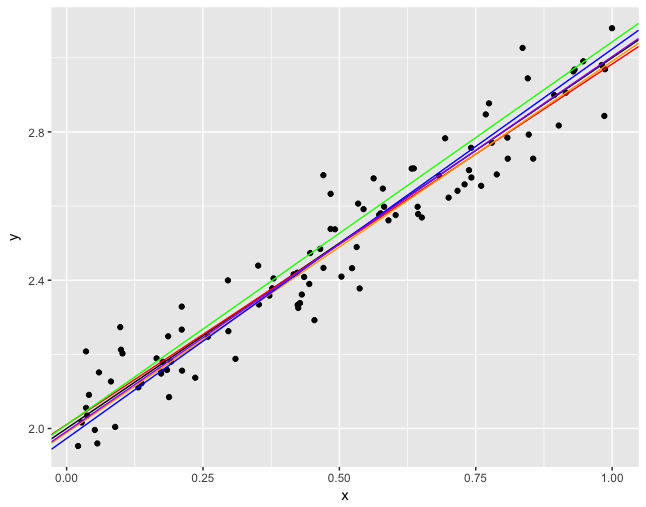
\includegraphics [height=6.5cm]{code/sca/sca+normal_0.1.png}
\caption{Fitted line Visualization, $\epsilon \sim \mathcal{N}(0,0.1)$, $n=100$}
\label{normal_0.1}
\end{center}

The second plot  Figure \ref{normal_1} uses noise $\sim \mathcal{N}(0,1)$. We can see that PLSE and HLSE give poor results due to they might maintain
 the horizontal distance, which will make $\hat{a}$ more large, VLSE give the best estimate because data distribution agree with its model assumption.

\begin{center}
\makeatletter
\def\@captype{figure}
\makeatother
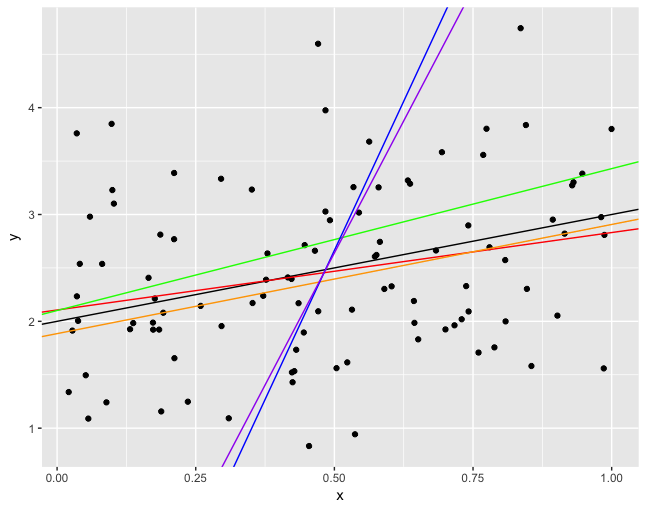
\includegraphics [height=6.5cm]{code/sca/sca+normal_1.png}
\caption{Fitted line Visualization, $\epsilon \sim \mathcal{N}(0,1)$, $n=100$}
\label{normal_1}
\end{center}

The third plot Figure \ref{cauchy} uses noise $\sim \mathrm{Cauchy}(0,0.2)$. Also, PLSE and HLSE give poor results due to they might maintain the horizontal distance, which will make $\hat{a}$ more large. VLME also give poor result because it want to maintain the extreme outliers (the top point). VLSE are also influenced by the outliers, while the VLAD are not influenced by the outliers.

\begin{center}
\makeatletter
\def\@captype{figure}
\makeatother
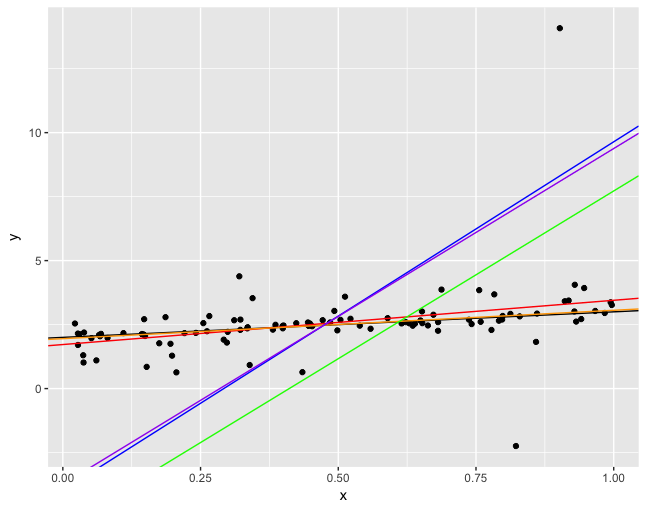
\includegraphics [height=6.5cm]{code/sca/sca+cauchy.png}
\caption{Fitted line Visualization, $\epsilon \sim \mathrm{Cauchy}(0,0.2)$, $n=100$}
\label{cauchy}
\end{center}

The last plot Figure \ref{uniform} use noise $\sim \mathcal{U}(-1,1)$. Ultimately, PLSE and HLSE still give poor results due to they might maintain the horizontal distance, which will make $\hat{a}$ more large. VLSE and VLAD provides ordinary performance and VLME offer the best results because it find the mid-point between the max and min, which well fit the data distribution.

\begin{center}
\makeatletter
\def\@captype{figure}
\makeatother
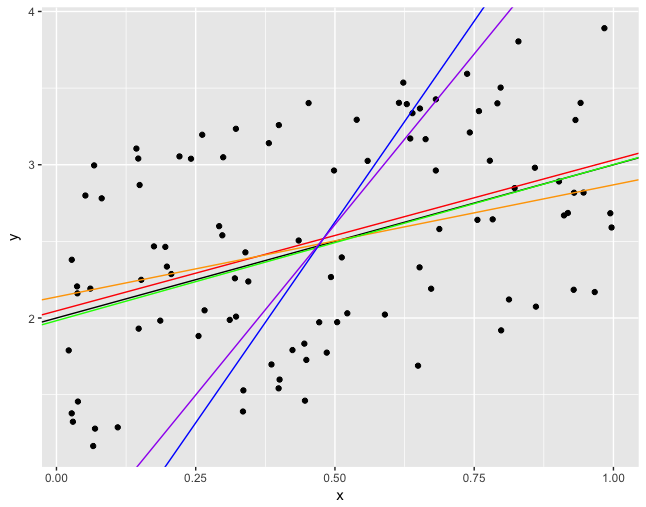
\includegraphics [height=6.5cm]{code/sca/sca+uniform.png}
\caption{Fitted line Visualization, $\epsilon \sim \mathcal{U}(-1,1)$, $n=100$}
\label{uniform}
\end{center}

\section{Appendix}

\subsection{All Experiments Results}
\label{append}

\begin{table}[ht]
\caption{uniform $X$, $\epsilon \sim \mathcal{N}(0,0.1)$}
\centering
\begin{tabular}{rlrrrr}
  \hline
  n & method & a.bias & a.sd & b.bias & b.sd \\ 
  \hline
  30 & VLAD & \textbf{0.001} & 0.084 & \textbf{-0.000} & 0.047 \\ 
  30 & VLSE & \textbf{0.001} & \textbf{0.064} & \textbf{-0.000} & \textbf{0.038} \\ 
  30 & VLME & 0.003 & 0.122 & -0.002 & 0.072 \\ 
  30 & HLSE & 0.122 & 0.067 & -0.061 & 0.040 \\ 
  30 & PLSE & 0.063 & 0.066 & -0.032 & 0.039 \\ 
  \hline
  100 & VLAD & 0.003 & 0.043 & \textbf{-0.001} & 0.025 \\ 
  100 & VLSE & \textbf{0.002} & \textbf{0.034} & \textbf{-0.001} & \textbf{0.020} \\ 
  100 & VLME & 0.003 & 0.098 & -0.002 & 0.058 \\ 
  100 & HLSE & 0.123 & 0.036 & -0.062 & 0.021 \\ 
  100 & PLSE & 0.064 & 0.036 & -0.033 & 0.021 \\ 
   \hline
  1000 & VLAD & \textbf{0.000} & 0.014 & \textbf{-0.000} & 0.008 \\ 
  1000 & VLSE & \textbf{-0.000} & \textbf{0.011} & \textbf{-0.000} & \textbf{0.006} \\ 
  1000 & VLME & 0.006 & 0.075 & -0.002 & 0.046 \\ 
  1000 & HLSE & 0.120 & 0.012 & -0.060 & 0.007 \\ 
  1000 & PLSE & 0.062 & 0.012 & -0.031 & 0.007 \\ 
   \hline
\end{tabular}
\end{table}

\begin{table}[ht]
\centering
\caption{uniform $X$, $\epsilon \sim \mathcal{N}(0,1)$}
\begin{tabular}{rlrrrr}
  \hline
 & method & a.bias & a.sd & b.bias & b.sd \\ 
  \hline
  30 & VLAD & \textbf{0.007} & 0.837 & \textbf{-0.000} & 0.474 \\ 
  30 & VLSE & 0.011 & \textbf{0.644} & -0.004 & \textbf{0.378} \\ 
  30 & VLME & 0.036 & 1.215 & -0.023 & 0.713 \\ 
  30 & HLSE & 24.476 & 440.576 & -12.071 & 222.122 \\ 
  30 & PLSE & 22.500 & 406.572 & -11.100 & 205.020 \\ 
   \hline
  100 & VLAD & 0.028 & 0.430 & \textbf{-0.013} & 0.250 \\ 
  100 & VLSE & \textbf{0.025} & \textbf{0.344} & -0.014 & \textbf{0.200} \\ 
  100 & VLME & 0.025 & 0.979 & -0.017 & 0.577 \\ 
  100 & HLSE & 15.178 & 27.934 & -7.580 & 13.259 \\ 
  100 & PLSE & 14.017 & 25.813 & -7.000 & 12.239 \\ 
   \hline
  1000 & VLAD & 0.005 & 0.142 & -0.003 & 0.080 \\ 
  1000 & VLSE & \textbf{-0.000} & \textbf{0.113} & \textbf{-0.001} & \textbf{0.063} \\ 
  1000 & VLME & 0.063 & 0.740 & -0.026 & 0.457 \\ 
  1000 & HLSE & 12.150 & 1.480 & -6.077 & 0.751 \\ 
  1000 & PLSE & 11.219 & 1.365 & -5.612 & 0.692 \\ 
   \hline
\end{tabular}
\end{table}


\begin{table}[ht]
\centering
\caption{uniform $X$, $\epsilon \sim \mathcal{N}(0,2)$}
\begin{tabular}{rlrrrr}
  \hline
 & method & a.bias & a.sd & b.bias & b.sd \\ 
  \hline
  30 & VLAD & \textbf{0.013} & 1.676 & \textbf{-0.000} & 0.947 \\ 
  30 & VLSE & 0.023 & \textbf{1.288} & -0.009 & \textbf{0.756} \\ 
  30 & VLME & 0.073 & 2.435 & -0.048 & 1.426 \\ 
  30 & HLSE & -43.076 & 1895.6 & 18.783 & 853.4 \\ 
  30 & PLSE & -42.164 & 1859.6 & 18.380 & 837.2 \\ 
  \hline
  100 & VLAD & 0.057 & 0.860 & \textbf{-0.026} & 0.500 \\ 
  100 & VLSE & \textbf{0.049} & \textbf{0.688} & -0.029 & \textbf{0.399} \\ 
  100 & VLME & 0.054 & 1.958 & -0.035 & 1.154 \\ 
  100 & HLSE & 81.204 & 928.103 & -40.192 & 462.922 \\ 
  100 & PLSE & 79.449 & 909.728 & -39.326 & 453.759 \\ 
  \hline
  1000 & VLAD & 0.009 & 0.284 & -0.007 & 0.160 \\ 
  1000 & VLSE & \textbf{-0.001} & \textbf{0.226} & \textbf{-0.001} & \textbf{0.127} \\ 
  1000 & VLME & 0.121 & 1.478 & -0.049 & 0.912 \\ 
  1000 & HLSE & 51.148 & 16.415 & -25.587 & 8.289 \\ 
  1000 & PLSE & 50.102 & 16.070 & -25.063 & 8.115 \\ 
  \hline
\end{tabular}
\end{table}

\begin{table}[ht]
\centering
\caption{uniform $X$, $\epsilon \sim \mathrm{Cauchy}(0,0.1)$}
\begin{tabular}{rlrrrr}
  \hline
 & method & a.bias & a.sd & b.bias & b.sd \\ 
  \hline
  30 & VLAD & -0.004 & \textbf{0.117} & \textbf{0.001} & \textbf{0.067 }\\ 
  30 & VLSE & \textbf{0.003} & 6.052 & -0.126 & 4.318 \\ 
  30 & VLME & -0.007 & 8.944 & -1.968 & 33.145 \\ 
  30 & HLSE & 32.848 & 768.75 & -17.232 & 422.26 \\ 
  30 & PLSE & 31.735 & 759.24 & -16.654 & 417.09 \\ 
  \hline
  100 & VLAD & \textbf{-0.000} & \textbf{0.057} & \textbf{-0.001} & \textbf{0.033} \\ 
  100 & VLSE & 0.72 & 20.48 & -0.52 & 13.63 \\ 
  100 & VLME & -1.43 & 46.81 & -8.07 & 215.15 \\ 
  100 & HLSE & -73.27 & 6359.5 & 29.28 & 3140.5 \\ 
  100 & PLSE & -72.63 & 6320.1 & 28.98 & 3121.9 \\ 
  \hline
  1000 & VLAD & \textbf{0.00} & \textbf{0.02} & \textbf{-0.00} & \textbf{0.01} \\ 
  1000 & VLSE & -0.86 & 17.71 & 0.09 & 5.16 \\ 
  1000 & VLME & 9.84 & 127.85 & -167.75 & 2875.86 \\ 
  1000 & HLSE & -945.37 & 35303. & 467.74 & 17710. \\ 
  1000 & PLSE & -946.17 & 35303. & 468.15 & 17710. \\ 
  \hline
\end{tabular}
\end{table}

\begin{table}[ht]
\centering
\caption{uniform $X$, $\epsilon \sim \mathcal{U}(-0.2,0.2)$}
\begin{tabular}{rlrrrr}
  \hline
 & method & a.bias & a.sd & b.bias & b.sd \\ 
  \hline
  30 & VLAD & \textbf{0.000} & 0.123 & \textbf{0.000} & 0.071 \\ 
  30 & VLSE & 0.001 & 0.077 & -0.001 & 0.045 \\ 
  30 & VLME & \textbf{-0.000} & \textbf{0.052} & \textbf{-0.000} & \textbf{0.030} \\ 
  30 & HLSE & 0.160 & 0.076 & -0.081 & 0.045 \\ 
  30 & PLSE & 0.083 & 0.079 & -0.042 & 0.046 \\
  \hline
  100 & VLAD & \textbf{0.001} & 0.070 & \textbf{0.000} & 0.040 \\ 
  100 & VLSE & \textbf{0.001} & 0.042 & \textbf{0.000} & 0.024 \\ 
  100 & VLME & \textbf{-0.001} & \textbf{0.017} & 0.001 & \textbf{0.010} \\ 
  100 & HLSE & 0.162 & 0.041 & -0.080 & 0.024 \\ 
  100 & PLSE & 0.085 & 0.043 & -0.041 & 0.024 \\  
  \hline
  1000 & VLAD & -0.001 & 0.022 & \textbf{0.000} & 0.013 \\ 
  1000 & VLSE & -0.001 & 0.013 & \textbf{0.000} & 0.007 \\ 
  1000 & VLME & \textbf{-0.000} & \textbf{0.002} & \textbf{0.000} & \textbf{0.001} \\ 
  1000 & HLSE & 0.159 & 0.013 & -0.080 & 0.008 \\ 
  1000 & PLSE & 0.083 & 0.013 & -0.041 & 0.008 \\ 
   \hline
\end{tabular}
\end{table}

\begin{table}[ht]
\caption{fixed $X$, $\epsilon \sim \mathcal{N}(0,0.1)$}
\centering
\begin{tabular}{rlrrrr}
  \hline
  n & method & a.bias & a.sd & b.bias & b.sd \\ 
  \hline
  30 & VLAD & -0.005 & 0.080 & 0.004 & 0.046 \\ 
  30 & VLSE & \textbf{-0.004} & \textbf{0.063} & \textbf{0.002} & \textbf{0.037} \\ 
  30 & VLME & \textbf{-0.004} & 0.115 & \textbf{0.002} & 0.070 \\ 
  30 & HLSE & 0.103 & 0.062 & -0.051 & 0.036 \\ 
  30 & PLSE & 0.051 & 0.064 & -0.025 & 0.037 \\ 
  \hline
  100 & VLAD & \textbf{-0.000} & 0.044 & 0.001 & 0.025 \\ 
  100 & VLSE & 0.001 & \textbf{0.035} & \textbf{-0.000} & \textbf{0.019} \\ 
  100 & VLME & \textbf{-0.000} & 0.094 & \textbf{0.000} & 0.056 \\ 
  100 & HLSE & 0.117 & 0.035 & -0.058 & 0.020 \\ 
  100 & PLSE & 0.061 & 0.036 & -0.030 & 0.020 \\ 
   \hline
  1000 & VLAD & \textbf{-0.000} & 0.014 & \textbf{0.000} & 0.008 \\ 
  1000 & VLSE & \textbf{-0.000} & \textbf{0.011} & \textbf{0.000} & \textbf{0.006} \\ 
  1000 & VLME & 0.003 & 0.075 & -0.001 & 0.046 \\ 
  1000 & HLSE & 0.120 & 0.011 & -0.060 & 0.006 \\ 
  1000 & PLSE & 0.061 & 0.011 & -0.031 & 0.006 \\ 
   \hline
\end{tabular}
\end{table}

\begin{table}[ht]
\centering
\caption{fixed $X$, $\epsilon \sim \mathcal{N}(0,1)$}
\begin{tabular}{rlrrrr}
  \hline
 & method & a.bias & a.sd & b.bias & b.sd \\ 
  \hline
  30 & VLAD & -0.052 & 0.799 & 0.041 & 0.456 \\ 
  30 & VLSE & \textbf{-0.038} & \textbf{0.627} & \textbf{0.022} & \textbf{0.366} \\ 
  30 & VLME & -0.043 & 1.149 & 0.018 & 0.697 \\ 
  30 & HLSE & 23.924 & 598.004 & -11.959 & 299.004 \\ 
  30 & PLSE & 21.547 & 548.961 & -10.770 & 274.483 \\ 
   \hline
  100 & VLAD & -0.002 & 0.435 & 0.006 & 0.249 \\ 
  100 & VLSE & 0.013 & \textbf{0.347} & -0.004 & \textbf{0.195} \\ 
  100 & VLME & \textbf{0.001} & 0.935 & \textbf{0.003} & 0.560 \\ 
  100 & HLSE & 13.800 & 10.903 & -6.898 & 5.456 \\ 
  100 & PLSE & 12.699 & 10.042 & -6.347 & 5.025 \\
   \hline
  1000 & VLAD & \textbf{-0.000} & 0.136 & \textbf{0.000} & 0.078 \\ 
  1000 & VLSE & -0.001 & \textbf{0.109} & \textbf{0.000} & \textbf{0.062} \\ 
  1000 & VLME & 0.032 & 0.754 & -0.011 & 0.461 \\ 
  1000 & HLSE & 12.123 & 1.366 & -6.062 & 0.685 \\ 
  1000 & PLSE & 11.193 & 1.255 & -5.597 & 0.629 \\ 
   \hline
\end{tabular}
\end{table}


\begin{table}[ht]
\centering
\caption{fixed $X$, $\epsilon \sim \mathcal{N}(0,2)$}
\begin{tabular}{rlrrrr}
  \hline
 & method & a.bias & a.sd & b.bias & b.sd \\ 
  \hline
  30 & VLAD & -0.105 & 1.599 & 0.082 & 0.912 \\ 
  30 & VLSE & \textbf{-0.076} & \textbf{1.254} & 0.044 & \textbf{0.732} \\ 
  30 & VLME & \textbf{-0.076} & 2.293 & \textbf{0.034} & 1.393 \\ 
  30 & HLSE & -17.635 & 627.34 & 8.824 & 313.653 \\ 
  30 & PLSE & -17.252 & 612.30 & 8.632 & 306.133 \\ 
  \hline
  100 & VLAD & \textbf{-0.004} & 0.871 & 0.012 & 0.498 \\ 
  100 & VLSE & 0.025 & \textbf{0.694} & -0.008 & \textbf{0.389} \\ 
  100 & VLME & -0.006 & 1.877 & \textbf{0.006} & 1.123 \\ 
  100 & HLSE & 43404 & 1370e3 & -21702 & 685050 \\ 
  100 & PLSE & 42450 & 1339e3 & -21225 & 669980 \\ 
  \hline
  1000 & VLAD & \textbf{-0.000} & 0.272 & \textbf{0.000} & 0.155 \\ 
  1000 & VLSE & -0.003 & \textbf{0.217} & \textbf{0.000} & \textbf{0.124} \\ 
  1000 & VLME & 0.074 & 1.496 & -0.025 & 0.916 \\ 
  1000 & HLSE & 50.611 & 12.981 & -25.307 & 6.492 \\ 
  1000 & PLSE & 49.574 & 12.711 & -24.788 & 6.357 \\ 
  \hline
\end{tabular}
\end{table}

\begin{table}[ht]
\centering
\caption{fixed $X$, $\epsilon \sim \mathrm{Cauchy}(0,0.1)$}
\begin{tabular}{rlrrrr}
  \hline
 & method & a.bias & a.sd & b.bias & b.sd \\ 
  \hline
  30 & VLAD & \textbf{0.002} & \textbf{0.108} & \textbf{-0.004} & \textbf{0.062} \\ 
  30 & VLSE & 0.139 & 9.132 & -0.096 & 6.586 \\ 
  30 & VLME & -0.063 & 7.436 & -0.185 & 34.296 \\ 
  30 & HLSE & -45.118 & 2467.1 & 22.533 & 1233.7 \\ 
  30 & PLSE & -44.808 & 2443.8 & 22.378 & 1222.0 \\ 
  \hline
  100 & VLAD & \textbf{-0.001} & \textbf{0.054} & \textbf{-0.001} & \textbf{0.031} \\ 
  100 & VLSE & 0.580 & 26.369 & -0.604 & 19.531 \\ 
  100 & VLME & 0.268 & 13.460 & -15.605 & 351.753 \\ 
  100 & HLSE & -22.683 & 2885.6 & 11.028 & 1447.11 \\ 
  100 & PLSE & -23.212 & 2884.3 & 11.292 & 1446.43 \\ 
  \hline
  1000 & VLAD & \textbf{-0.001} & \textbf{0.017} & \textbf{0.001} & \textbf{0.010} \\ 
  1000 & VLSE & -1.667 & 26.787 & 0.423 & 11.228 \\ 
  1000 & VLME & 15.23 & 781.16 & -207.35 & 5981.57 \\ 
  1000 & HLSE & -4363.2 & 70387 & 2181.2 & 35184 \\ 
  1000 & PLSE & -4363.6 & 70384 & 2181.4 & 35182 \\ 
  \hline
\end{tabular}
\end{table}

\begin{table}[ht]
\centering
\caption{fixed $X$, $\epsilon \sim \mathcal{U}(-0.2,0.2)$}
\begin{tabular}{rlrrrr}
  \hline
 & method & a.bias & a.sd & b.bias & b.sd \\ 
  \hline
  30 & VLAD & -0.008 & 0.113 & 0.006 & 0.066 \\ 
  30 & VLSE & -0.003 & 0.070 & 0.003 & 0.040 \\ 
  30 & VLME & \textbf{0.000} & \textbf{0.046} & \textbf{-0.000} & \textbf{0.026} \\ 
  30 & HLSE & 0.138 & 0.066 & -0.068 & 0.038 \\ 
  30 & PLSE & 0.069 & 0.071 & -0.033 & 0.041 \\ 
  \hline
  100 & VLAD & 0.002 & 0.069 & 0.001 & 0.039 \\ 
  100 & VLSE & 0.001 & 0.041 & 0.000 & 0.023 \\ 
  100 & VLME & \textbf{0.000} & \textbf{0.016} & \textbf{-0.000} & \textbf{0.009} \\ 
  100 & HLSE & 0.156 & 0.038 & -0.077 & 0.022 \\ 
  100 & PLSE & 0.081 & 0.042 & -0.040 & 0.024 \\ 
  \hline
  1000 & VLAD & 0.001 & 0.022 & -0.001 & 0.012 \\ 
  1000 & VLSE & 0.001 & 0.012 & -0.000 & 0.007 \\ 
  1000 & VLME & \textbf{-0.000} & \textbf{0.002} & \textbf{0.000} & \textbf{0.001} \\ 
  1000 & HLSE & 0.160 & 0.012 & -0.080 & 0.007 \\ 
  1000 & PLSE & 0.084 & 0.013 & -0.042 & 0.007 \\ 
   \hline
\end{tabular}
\end{table}

\end{document}
